\documentclass[10pt,journal,compsoc]{IEEEtran}

\usepackage[T1]{fontenc}
\usepackage[utf8]{inputenc}

\usepackage{acronym} % \ac[p], \acl[p], \acs[p], \acf[p]

\usepackage[nocompress]{cite}

\usepackage[pdftex]{graphicx}
\graphicspath{{img/}}
\DeclareGraphicsExtensions{.pdf,.jpeg,.png}
\usepackage{color}
\AtBeginDocument{
\definecolor{pdfurlcolor}{rgb}{0,0,0}
\definecolor{pdfcitecolor}{rgb}{0,0,0}
\definecolor{pdflinkcolor}{rgb}{0,0,0}
\definecolor{light}{gray}{.85}
\definecolor{vlight}{gray}{.95}
\definecolor{darkgreen}{rgb}{0.0, 0.2, 0.13}
\definecolor{mydarkblue}{RGB}{116,173,209}
\definecolor{mydarkblueid}{RGB}{83,154,198}
\definecolor{mylightblue}{RGB}{171,217,233}
\definecolor{mydarkorange}{RGB}{244,109,67}
\definecolor{mylightorange}{RGB}{252,153,54}
\definecolor{mydarkred}{RGB}{215,48,39}
\definecolor{mydarkpurple}{RGB}{140,107,177}
\definecolor{mydarkpurpleid}{RGB}{136,86,167}
}

\usepackage{amsmath}
\interdisplaylinepenalty=2500
\newtheorem{myrule}{Rule}
\def\algorithmautorefname{Algorithm} % \autoref
\def\myruleautorefname{Rule} % \autoref

\usepackage{algorithmic}
\renewcommand{\algorithmicrequire}{\textbf{Input:}}
\renewcommand{\algorithmicensure}{\textbf{Output:}}

% algorithmic.sty was written by Peter Williams and Rogerio Brito.
% This package provides an algorithmic environment fo describing algorithms.
% You can use the algorithmic environment in-text or within a figure
% environment to provide for a floating algorithm. Do NOT use the algorithm
% floating environment provided by algorithm.sty (by the same authors) or
% algorithm2e.sty (by Christophe Fiorio) as the IEEE does not use dedicated
% algorithm float types and packages that provide these will not provide
% correct IEEE style captions. The latest version and documentation of
% algorithmic.sty can be obtained at:
% http://www.ctan.org/pkg/algorithms
% Also of interest may be the (relatively newer and more customizable)
% algorithmicx.sty package by Szasz Janos:
% http://www.ctan.org/pkg/algorithmicx

\usepackage{booktabs} % \toprule, \midrule, \cmidrule, \bottomrule
\usepackage[inline]{enumitem} % \begin{enumerate*} \end{enumerate*}
\usepackage{tikz} % \begin{tikzpicture} \end{tikzpicture}
\usetikzlibrary{shapes.misc}

\usepackage[caption=false,font=footnotesize,labelfont=sf,textfont=sf]{subfig}

\usepackage{dblfloatfix}

\ifCLASSOPTIONcaptionsoff
 \usepackage[nomarkers]{endfloat}
\let\MYoriglatexcaption\caption
\renewcommand{\caption}[2][\relax]{\MYoriglatexcaption[#2]{#2}}
\fi

% \usepackage{url}
\usepackage{hyperref}

\usepackage[draft,inline,nomargin,index]{fixme}
\fxsetup{theme=colorsig,mode=multiuser,inlineface=\itshape,envface=\itshape}
\FXRegisterAuthor{go}{ago}{Gerald}
\FXRegisterAuthor{mn}{amn}{Matthieu}

% Commands
%---------
\newcommand{\ie}{i.e. }

\newcommand{\inbb}[1]{\in \mathbb{#1}}
\newcommand{\mathlist}[2]{\set{#1_i \in #2}_{i \inbb{N}}}
\newcommand{\new}{\textbf{new}}
\newcommand{\trm}[1]{\mathit{#1}}
\newcommand{\set}[1]{\left\{#1\right\}} % set brace notation

\newcommand{\id}[3]{$\trm{#1}^{\trm{#2}}_{\trm{#3}}$}
\newcommand{\epoch}[1]{$\varepsilon_{#1}$}

\newcommand{\widthletter}{2em}
\newcommand{\widthblock}{3em}
\newcommand{\widthoriginepoch}{1.65em}
\newcommand{\widthepoch}{1.8em}

% Tikz styles
\tikzset{
    common/.style={anchor=west, draw, rectangle, minimum height=6mm},
    letter/.style={common, minimum width=\widthletter},
    block/.style={common, minimum width=\widthblock},
    epoch/.style={letter, rounded rectangle, rounded rectangle east arc=0pt, minimum width=\widthepoch},
    op/.style={draw, circle, minimum size=2em},
    causalop/.style={op, double=white, inner sep=2pt},
    cross/.style={
        path picture={
            \draw[mydarkred, very thick]
                (path picture bounding box.south east)--(path picture bounding box.north west)
                (path picture bounding box.south west)--(path picture bounding box.north east);
        }
    }
}

% Acronyms
% --------
\acrodef{ADT}[ADT]{Abstract Data Type}
\acrodefplural{ADT}[ADTs]{Abstract Data Types}
\acrodef{CRDT}[CRDT]{Conflict-free Replicated Data Type}
\acrodefplural{CRDT}[CRDTs]{Conflict-free Replicated Data Types}
\acrodef{EC}[EC]{Eventual Consistency}
\acrodef{JIT}[JIT]{Just-In-Time}
\acrodef{LCA}[LCA]{Lowest Common Ancestor}
\acrodef{OT}[OT]{Operational Transformation}
\acrodefplural{OT}[OT]{Operational Transformations}
\acrodef{P2P}[P2P]{Peer-to-Peer}
\acrodef{SEC}[SEC]{Strong Eventual Consistency}

% correct bad hyphenation here
\hyphenation{op-tical net-works semi-conduc-tor Renamable-LogootSplit}

\begin{document}

\title{Efficient Renaming in Sequence CRDTs}

\author{Matthieu~Nicolas, %~\IEEEmembership{Member,~IEEE,}
        Gérald~Oster %~\IEEEmembership{Fellow,~OSA,}
        and~Olivier~Perrin%~\IEEEmembership{Life~Fellow,~IEEE}% <-this % stops a space
\IEEEcompsocitemizethanks{\IEEEcompsocthanksitem The authors are with the Université de Lorraine, CNRS, Inria, LORIA, F-54500, Nancy, France.\protect\\
% note need leading \protect in front of \\ to get a newline within \thanks as
% \\ is fragile and will error, could use \hfil\break instead.
E-mail: \{matthieu.nicolas, gerald.oster, olivier.perrin\}@loria.fr.}% <-this % stops an unwanted space
\thanks{Manuscript received ???; revised ???.}}

% The paper headers
%\markboth{Journal of \LaTeX\ Class Files,~Vol.~14, No.~8, August~2015}%
%{Shell \MakeLowercase{\textit{et al.}}: Bare Demo of IEEEtran.cls for Computer Society Journals}
% The only time the second header will appear is for the odd numbered pages
% after the title page when using the twoside option.
%
% *** Note that you probably will NOT want to include the author's ***
% *** name in the headers of peer review papers.                   ***
% You can use \ifCLASSOPTIONpeerreview for conditional compilation here if
% you desire.



% The publisher's ID mark at the bottom of the page is less important with
% Computer Society journal papers as those publications place the marks
% outside of the main text columns and, therefore, unlike regular IEEE
% journals, the available text space is not reduced by their presence.
% If you want to put a publisher's ID mark on the page you can do it like
% this:
%\IEEEpubid{0000--0000/00\$00.00~\copyright~2015 IEEE}
% or like this to get the Computer Society new two part style.
%\IEEEpubid{\makebox[\columnwidth]{\hfill 0000--0000/00/\$00.00~\copyright~2015 IEEE}%
%\hspace{\columnsep}\makebox[\columnwidth]{Published by the IEEE Computer Society\hfill}}
% Remember, if you use this you must call \IEEEpubidadjcol in the second
% column for its text to clear the IEEEpubid mark (Computer Society jorunal
% papers don't need this extra clearance.)

% for Computer Society papers, we must declare the abstract and index terms
% PRIOR to the title within the \IEEEtitleabstractindextext IEEEtran
% command as these need to go into the title area created by \maketitle.
% As a general rule, do not put math, special symbols or citations
% in the abstract or keywords.
\IEEEtitleabstractindextext{%
\begin{abstract}
The abstract goes here.
\end{abstract}

% Note that keywords are not normally used for peerreview papers.
\begin{IEEEkeywords}
CRDTs, real-time collaborative editing, eventual consistency, memory-wise optimisation, performance.
\end{IEEEkeywords}}

% make the title area
\maketitle

% For peer review papers, you can put extra information on the cover
% page as needed:
% \ifCLASSOPTIONpeerreview
% \begin{center} \bfseries EDICS Category: 3-BBND \end{center}
% \fi
%
% For peerreview papers, this IEEEtran command inserts a page break and
% creates the second title. It will be ignored for other modes.
\IEEEpeerreviewmaketitle

\IEEEraisesectionheading{\section{Introduction}\label{sec:introduction}}
% The very first letter is a 2 line initial drop letter followed
% by the rest of the first word in caps (small caps for compsoc).
%
% form to use if the first word consists of a single letter:
% \IEEEPARstart{A}{demo} file is ....
%
% form to use if you need the single drop letter followed by
% normal text (unknown if ever used by the IEEE):
% \IEEEPARstart{A}{}demo file is ....
%
% Some journals put the first two words in caps:
% \IEEEPARstart{T}{his demo} file is ....
%
% Here we have the typical use of a "T" for an initial drop letter
% and "HIS" in caps to complete the first word.
\IEEEPARstart{T}{his} demo file is intended to serve as a ``starter file''
for IEEE Computer Society journal papers produced under \LaTeX\ using
IEEEtran.cls version 1.8b and later.
% You must have at least 2 lines in the paragraph with the drop letter
% (should never be an issue)
I wish you the best of success.

% needed in second column of first page if using \IEEEpubid
%\IEEEpubidadjcol

\section{Background}
\label{sec:background}

To deterministically solve conflicts and ensure convergence of all nodes, \acp{CRDT} rely on metadata.
In the context of Sequence \acp{CRDT}, two different approaches were proposed, both trying to minimise the overhead introduced.
The first one \cite{oster:inria-00108523, ROH2011354,briot:hal-01343941} attaches fixed size identifiers to each element in the sequence and uses them to represent the sequence as a linked list.
The downside of this approach is an ever growing overhead, as it needs to keep removed elements to deal with potential concurrent updates, effectively turning them into tombstones.
The second one \cite{5158449,WeissICDCS09,weiss:hal-00450416,AndreCollaborateCom2013,nedelec_2013_lseq,doi:10.1002/cpe.4108} avoids the need of tombstones by attaching identifiers from a dense totally ordered set to elements.
Elements are ordered into the sequence by comparing their respective identifiers.
However this approach suffers from an ever-increasing overhead, as the size of such dense totally ordered identifiers is variable and grows over time.
In the context of this paper, we focus on the later approach.


\subsection{LogootSplit}

LogootSplit (LS) \cite{AndreCollaborateCom2013} is the state of the art of the variable-size identifiers approach of Sequence \ac{CRDT}.
As explained previously, it uses identifiers from a dense totally ordered set to position elements into the replicated sequence.

To this end, LogootSplit generates identifiers made of a list of tuples to elements.
These tuples have four components:
\begin{enumerate*}
    \item a \emph{position}, which embodies the intended position of the element
    \item a \emph{node identifier},
    \item a \emph{node sequence number} and
    \item an \emph{offset}, which are combined to make identifiers unique.
\end{enumerate*}
By comparing identifiers using the lexicographical order, LogootSplit is able to determine the position of the element relatively to others.
In this paper, we represent identifiers using the following notation: \id{position}{node~id~node~seq}{offset} where $\trm{position}$ is a lowercase letter, $\trm{node~id}$ an uppercase one and both $\trm{node~seq}$ and $\trm{offset}$ integers.

Instead of storing an identifier for each element of the sequence, the main insight of LogootSplit is to aggregate dynamically elements into blocks.
Grouping elements into blocks enables LogootSplit to assign logically an identifier to each element while effectively storing only the block length and the identifier of its first element.
LogootSplit gathers elements with \emph{contiguous} identifiers into a block.
We call \emph{contiguous} two identifiers that are identical except for their last offset, and with both offsets being consecutive.
\autoref{fig:logootsplit-seq} illustrates such a case: in \autoref{fig:logootsplit-seq-as-letters}, the element identifiers form a chain of contiguous identifiers.
LogootSplit is then able to group them into one block to minimise the metadata stored, as shown in \autoref{fig:logootsplit-seq-as-block}.

\begin{figure}[!t]
    \centering
    \subfloat[Elements with their corresponding identifiers]{
        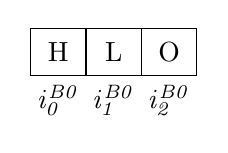
\begin{tikzpicture}
            \path
                node[letter, label=below:{\id{i}{B0}{0}}] {H}
                to ++(0:\widthletter) node[letter, label=below:{\id{i}{B0}{1}}] {L}
                to ++(0:\widthletter) node[letter, label=below:{\id{i}{B0}{2}}] {O};
        \end{tikzpicture}
        \label{fig:logootsplit-seq-as-letters}}
    \hfil
    \subfloat[Elements grouped into a block]{
        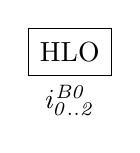
\begin{tikzpicture}
            \path
                node[block, label=below:{\id{i}{B0}{0..2}}] {HLO};
        \end{tikzpicture}
        \label{fig:logootsplit-seq-as-block}}
    \caption{Simulation results for the network.}
    \label{fig:logootsplit-seq}
\end{figure}

This feature allows to shift the root of metadata growth from the number of elements to the number of blocks.
As blocks can contain an arbitrary number of elements, it enables to reduce significantly the memory overhead of the data structure.

\subsection{Limits}

As stated previously, the size of identifiers from a dense totally ordered set is variable.
When nodes insert new elements between two others with the same \emph{position} value, LogootSplit has no other option than to increase the size of the resulting identifiers.
\autoref{fig:example-split} illustrates such cases.
In this example, since the node inserts a new element between contiguous identifiers, LogootSplit is not able to generate a fitting identifier of the same size.
To comply with the intended order, LogootSplit generates a new identifier by appending a new tuple to the identifier of the predecessor.

\begin{figure}[t!]
    \centering
    \begin{tikzpicture}
        \path
            node {\textbf{A}}
            to ++(0:\widthletter) node[block, label=below:{\id{i}{B0}{0..2}}] (HLO) {HLO}
            to ++(0:5 * \widthletter) node[letter, label=below:{\id{i}{B0}{0}}] (H) {H}
            to ++(0:\widthletter) node[letter, fill=mydarkorange, label=above:{\color{mydarkorange}\id{i}{B0}{0}\id{f}{A0}{0}}] {E}
            to ++(0:\widthletter) node[block, label=below:{\id{i}{B0}{1..2}}] {LO};

        \draw[->, thick] (HLO) -- node[below, align=center]{\emph{insert "e"}\\\emph{between}\\\emph{"h" and "l"}} (H);
    \end{tikzpicture}
    \caption{Insertion leading to longer identifiers}
    \label{fig:example-split}
\end{figure}

As a result, the size of identifiers tends to grow as the collaboration progresses.
This growth impacts negatively performance of the data structure on several aspects.
Since identifiers attached to values become longer, the memory overhead of the data structure increases accordingly.
This also increases the bandwidth consumption as nodes have to broadcast identifiers to others.

Additionally, as the lifetime of the replicated sequence increases, the number of blocks composing it grows as well.
Indeed, several constraints on identifier generation prevent nodes from adding new elements to existing blocks.
For example, only the node that generated the block can append or prepend elements to it.
These limitations cause the generation of new blocks.
Since no mechanism to merge blocks a posteriori is provided, the sequence ends up fragmented into many blocks.
The efficiency of the data structure decreases as each block introduces its own overhead.

In our benchmarks, we measure that the content eventually represents less than 1\% of the data structure size, the remaining 99\% being metadata.
It is thus necessary to address the previously highlighted issues.

\section{Overview}
\label{sec:overview}

\subsection{Proposed approach}
\label{sec:proposition}

We propose a new Sequence \ac{CRDT} belonging to the variable-size identifiers approach: \emph{RenamableLogootSplit} (RLS) \cite{nicolas:hal-01932552}.

To address the limitations of LogootSplit, we embed in the data structure a renaming mechanism.
The purpose of this mechanism is to reassign shorter identifiers to elements and to group them into blocks to minimise the memory overhead of the whole sequence.

To avoid costly and blocking consensus algorithms, we instead adopt the \emph{optimistic replication} \cite{10.1145/1057977.1057980} approach for our mechanism.
Nodes perform renaming without any coordination.
However, this operation is not intrinsically commutative with others.
If conflicts arise, we use \emph{Operational Transformations} (OT) \cite{10.1145/289444.289469,4668339} to enable nodes to resolve them deterministically.

\subsection{System Model}

The system is composed of a dynamic set of nodes, as nodes join and leave dynamically the collaboration during its lifetime.
Nodes collaborate to build and maintain a sequence using RenamableLogootSplit.
Each node owns a copy of the sequence and edit it without any coordination.

Nodes communicate through a \ac{P2P} network, which is unreliable.
Messages can be lost, re-ordered or delivered multiple times.
The network is also vulnerable to partitions, which split nodes into disjoined subgroups.
To overcome the failures of the network, nodes rely on a message-passing layer.
As RenamableLogootSplit is built on top of LogootSplit, it shares the same requirements for the operation delivery.
This layer is thus used to deliver messages to the application exactly-once.
The layer also ensures that \emph{remove} operations are delivered after corresponding \emph{insert} operations.
Nodes use an anti-entropy mechanism to synchronise in a pairwise manner, by detecting and re-exchanging lost operations.

\section{RenamableLogootSplit in centralised settings}
\label{sec:centralised-rls}

\subsection{\emph{rename} operation}

\label{sec:rename-op}

Our \emph{rename} operation helps RenamableLogootSplit to reduce the overhead of nodes replica.
This operation reassigns arbitrary identifiers to elements.

\begin{figure}[t!]
    \centering
    \subfloat[Selecting the new identifier of the first element]{
        \begin{tikzpicture}
            \path
                node {\textbf{A}}
                to ++(0:\widthletter) node[letter, label=below:{\id{i}{B0}{0}}] {H}
                to ++(0:\widthletter) node[letter, fill=mydarkorange, label=above:{\color{mydarkorange}\id{i}{B0}{0}\id{f}{A0}{0}}] {E}
                to ++(0:\widthletter) node[block, label=below:{\id{i}{B0}{1..2}}] (LO) {LO}
                to ++(0:4 * \widthletter) node[letter, fill=mydarkblue, label=below:{\color{mydarkblueid}\id{i}{A1}{0}}] (H) {H};

            \draw[->, thick] (LO) -- node[below, align=center]{\emph{rename}} (H);
        \end{tikzpicture}
        \label{fig:renaming-first-id}}
    \hfil
    \subfloat[Selecting the new identifiers of the remaining ones]{
        \begin{tikzpicture}
            \path
                node {\textbf{A}}
                to ++(0:\widthletter) node[letter, label=below:{\id{i}{B0}{0}}] {H}
                to ++(0:\widthletter) node[letter, fill=mydarkorange, label=above:{\color{mydarkorange}\id{i}{B0}{0}\id{f}{A0}{0}}] {E}
                to ++(0:\widthletter) node[block, label=below:{\id{i}{B0}{1..2}}] (LO) {LO}
                to ++(0:4 * \widthletter) node[letter, fill=mydarkblue, label=below:{\color{mydarkblueid}\id{i}{A1}{0}}] (H) {H}
                to ++(0:\widthletter) node[letter, fill=mydarkblue, label=below:{\color{mydarkblueid}\id{i}{A1}{1}}] {E}
                to ++(0:\widthletter) node[letter, fill=mydarkblue, label=below:{\color{mydarkblueid}\id{i}{A1}{2}}] {L}
                to ++(0:\widthletter) node[letter, fill=mydarkblue, label=below:{\color{mydarkblueid}\id{i}{A1}{3}}] {0};

                \draw[->, thick] (LO) -- node[below, align=center]{\emph{rename}} (H);
            \end{tikzpicture}
        \label{fig:renaming-second-id}}
    \hfil
    \subfloat[Final state obtained]{
        \begin{tikzpicture}
            \path
                node {\textbf{A}}
                to ++(0:\widthletter) node[letter, label=below:{\id{i}{B0}{0}}] {H}
                to ++(0:\widthletter) node[letter, fill=mydarkorange, label=above:{\color{mydarkorange}\id{i}{B0}{0}\id{f}{A0}{0}}] {E}
                to ++(0:\widthletter) node[block, label=below:{\id{i}{B0}{1..2}}] (LO) {LO}
                to ++(0:4 * \widthletter) node[block, fill=mydarkblue, label=below:{\color{mydarkblueid}\id{i}{A1}{0..3}}] (HELO) {HELO};

            \draw[->, thick] (LO) -- node[below, align=center]{\emph{rename}} (HELO);
        \end{tikzpicture}
        \label{fig:renaming-final-state}}
    \caption{Renaming the sequence on node \emph{A}}
    \label{fig:renaming}
\end{figure}


Its behaviour is illustrated in \autoref{fig:renaming}.
In this example, node A initiates a \emph{rename} operation on its local state.
First, node A reuses the id of the first element of the sequence (\id{i}{B0}{0}) but modifies it with its own node id (\textbf{A}) and current sequence number (\emph{1}).
Also the offset is set to 0.
Node A reassigns the resulting id (\id{i}{A1}{0}) to the first element of the sequence as described in \autoref{fig:renaming-first-id}.
Then, node A derives contiguous identifiers for all remaining elements by successively incrementing the offset (\id{i}{A1}{1}, \id{i}{A1}{2} and \id{i}{A1}{3}), as shown in \autoref{fig:renaming-second-id}.
As we assign contiguous identifiers to all elements of the sequence, we eventually group them into one block as illustrated in \autoref{fig:renaming-final-state}.
It allows nodes to benefit the most from the block feature and to minimise the overhead of the resulting state.

To eventually converge, other nodes have to rename their state identically.
However, they can not simply replace their current state with the new renamed one.
Indeed, they may have performed concurrent updates on their states.
To not discard these updates, nodes have to process the \emph{rename} operation themselves.
To this end, the node issuing the \emph{rename} operation broadcasts its former state to others.
Using the former state, other nodes compute the new identifier of each renamed identifier.
As for concurrently inserted identifiers, we will explain in \autoref{sec:dealing-with-concurrent-updates} how nodes rename them in a deterministic way.

To limit bandwidth consumption of \emph{rename} operations, we propose a compression technique to broadcast only necessary components to uniquely identify blocks instead of whole identifiers.
It reduces the data to send to a fixed amount per block.
Additionally, we can set an upper-bound to the size of \emph{rename} operations by issuing them as soon as the state reaches a given number of blocks.

\subsection{Dealing with concurrent updates}

\label{sec:dealing-with-concurrent-updates}

As \emph{rename} operations can be issued without any kind of coordination, it is possible for other nodes to perform updates concurrently.
Figure \ref{fig:concurrent-insert-rename-inconsistent} illustrates such cases.
In this example node B inserts the new element "L", assigns the id \id{i}{B0}{0}\id{m}{B1}{0} to it and broadcasts its update, concurrently to the \emph{rename} operation described in \autoref{fig:renaming}.
Upon reception of the \emph{insert} operation, node A adds the inserted element into its sequence, using the element id to determine its position.
However, since identifiers were modified by the concurrent \emph{rename} operation, node A inserts the new element at the end of its sequence (since \id{i}{A1}{3} < \id{i}{B0}{0}\id{m}{B1}{0}) instead of at the intended position.
As described by this example, applying naively concurrent updates would result in inconsistencies.
It is thus necessary to handle concurrent operations to \emph{rename} operations in a particular manner.

\begin{figure}[t!]
    \centering
    \begin{tikzpicture}
        \path
            node[label=below:{(after renaming)}] {\textbf{A}}
            to ++(0:2 * \widthletter) node[block, fill=mydarkblue, label=below:{\color{mydarkblueid}\id{i}{A1}{0..3}}] (HELO) {HELO}
            to ++(0:4 * \widthletter) node[block, fill=mydarkblue, label=below:{\color{mydarkblueid}\id{i}{A1}{0..3}}]  {HELO}
            to ++(0:\widthblock) node[cross, letter, fill=mylightorange, label=above:{\color{mylightorange}\id{i}{B0}{0}\id{m}{B1}{0}}] (right) {L};

        \path
            to ++(270:2) node[label=below:{(before renaming)}]  {\textbf{B}}
            to ++(0:2*\widthletter) node[letter, label=below:{\id{i}{B0}{0}}] {H}
            to ++(0:\widthletter) node[letter, fill=mydarkorange, label=above:{\color{mydarkorange}\id{i}{B0}{0}\id{f}{A0}{0}}] {E}
            to ++(0:\widthletter) node[letter, fill=mylightorange, label=below:{\color{mylightorange}\id{i}{B0}{0}\id{m}{B1}{0}}] (left) {L}
            to ++(0:\widthletter) node[block, label=below:{\id{i}{B0}{1..2}}] {LO};

        \draw[dashed, ->, thick] (left.north) .. controls +(90:2 * \widthletter) and +(270:2 * \widthletter) .. node[below right, align=center]{\emph{insert}} (right.south);
    \end{tikzpicture}
    \caption{Concurrent update leading to inconsistency}
    \label{fig:concurrent-insert-rename-inconsistent}
\end{figure}

To detect them, we use an \emph{epoch-based} system.
We add an \emph{epoch} to the sequence as a property.
Each time a \emph{rename} operation is applied, the sequence progresses to a new epoch.
When nodes issue operations, they tag them with their current epoch.
Upon the reception of an operation, nodes compare the operation epoch to their current one.
If they differ, nodes have to transform the operation before applying it.

\autoref{alg:renameId} enables nodes to transform \emph{insert} or \emph{remove} operations against the \emph{rename} one.
The main idea of this algorithm is to use the predecessor of the given identifier to do so.
An example of its usage is illustrated in \autoref{fig:concurrent-insert-rename-fixed}.
This figure depicts the same scenario as in \autoref{fig:concurrent-insert-rename-inconsistent}, except that this time node A uses \autoref{alg:renameId} to rename the concurrently generated id before inserting it in its state.
The algorithm proceeds as follows.
First, node A retrieves the predecessor of the given id \id{i}{B0}{0}\id{m}{B1}{0} in the former state: \id{i}{B0}{0}\id{f}{A0}{0}.
Then it computes the counterpart of \id{i}{B0}{0}\id{f}{A0}{0} in the renamed state: \id{i}{A1}{1}.
Finally, node A prepends it to the given id to generate the renamed id: \id{i}{A1}{1}\id{i}{B0}{0}\id{m}{B1}{0}.
By reassigning this id to the concurrently added element, node A is able to insert it in its state while preserving the intended order.

\begin{figure}[t!]
    \centering
    \begin{tikzpicture}
        \path
            node[label=below:{(epoch 1)}] {\textbf{A}}
            to ++(0:2 * \widthletter) node[block, fill=mydarkblue, label=below:{\color{mydarkblueid}\id{i}{A1}{0..3}}] (HELO) {HELO}
            to ++(0:4 * \widthletter) node[block, fill=mydarkblue, label=below:{\color{mydarkblueid}\id{i}{A1}{0..1}}]  {HE}
            to ++(0:\widthblock) node[letter, fill=mylightblue, label=above:{\color{mylightblue!20!mydarkblueid}\id{i}{A1}{1}\id{i}{B0}{0}\id{m}{B1}{0}}] (right) {L}
            to ++(0:\widthletter) node[block, fill=mydarkblue, label=below:{\color{mydarkblueid}\id{i}{A1}{2..3}}]  {LO};


        \path
            to ++(270:2) node[label=below:{(epoch 0)}] {\textbf{B}}
            to ++(0:1.5 * \widthletter) node[letter, label=below:{\id{i}{B0}{0}}] {H}
            to ++(0:\widthletter) node[letter, fill=mydarkorange, label=above:{\color{mydarkorange}\id{i}{B0}{0}\id{f}{A0}{0}}] {E}
            to ++(0:\widthletter) node[letter, fill=mylightorange, label=below:{\color{mylightorange}\id{i}{B0}{0}\id{m}{B1}{0}}] (left) {L}
            to ++(0:\widthletter) node[block, label=below:{\id{i}{B0}{1..2}}] {LO};

        \draw[dashed, ->, thick] (left.north) .. controls +(90:2 * \widthletter) and +(270:2 * \widthletter) .. node[below right, align=center]{\emph{rename}\\ \emph{then insert}}(right.south);
    \end{tikzpicture}
    \caption{Renaming concurrent update using \autoref{alg:renameId} before applying it to maintain intended order}
    \label{fig:concurrent-insert-rename-fixed}
\end{figure}

\begin{figure}
    \begin{algorithmic}
        \REQUIRE id, renamedBlocks, nId, nSeq
        \ENSURE renamedId

        % \Statex \LeftComment{$\trm{id}$ is the identifier to rename}
        % \Statex \LeftComment{$\trm{renamedBlocks}$ is the former state}
        % \Statex \LeftComment{$\trm{nId}$ is $\trm{node~id}$ of the node which issued the \emph{rename} op}
        % \Statex \LeftComment{$\trm{nSeq}$ is $\trm{node~seq}$ of the node which issued the \emph{rename} op}\\

        \STATE length $\gets$ renamedBlocks.length
        \STATE firstId $\gets$ idBegin(renamedBlocks[0])
        \STATE lastId $\gets$ idEnd(renamedBlocks[length - 1])

        \STATE pos $\gets$ position(firstId)
        \STATE newFirstId $\gets$ \new~Id(pos, nId, nSeq, 0)
        \STATE newLastId $\gets$ \new~Id(pos, nId, nSeq, length - 1)

        \IF{firstId < id \AND id < lastId}
            \STATE pred $\gets$ findPredecessor(id, renamedBlocks)
            \STATE indexOfPred $\gets$ findIndex(pred, renamedBlocks)
            \STATE newPred $\gets$ \new~Id(pos, nId, nSeq, indexOfPred)
            \RETURN concat(newPredecessor, id)
        \ELSIF{lastId < id \AND id < newLastId}
            \RETURN concat(newLastId, id)
        \ELSIF{newFirstId < id \AND id < firstId}
            \STATE predOfNewFirstId $\gets$ \new~Id(pos, nId, nSeq, -1)
            \RETURN concat(predOfNewFirstId, id)
        \ELSE
            \RETURN id \COMMENT{Return the identifier unchanged as it does not conflict with the rename op}
        \ENDIF
    \end{algorithmic}
    \caption{Rename concurrently generated identifier}
    \label{alg:renameId}
\end{figure}

As explained in \autoref{sec:rename-op}, some nodes may have applied concurrent \emph{insert} operations to their state before receiving a given remote \emph{rename} operation.
\autoref{alg:renameId} also solves this case.
It allows them to eventually converge with nodes which processed the \emph{rename} operations before the concurrent \emph{insert} operations.

Since nodes rely on the former state to transform concurrent operations to a \emph{rename} one, they have to store it.
Nodes need it until each of them can no longer issue concurrent operations to the corresponding \emph{rename} operation.
In other words, nodes can safely garbage collect the former state once the \emph{rename} operation became causally stable \cite{10.1007/978-3-662-43352-2_11}.
Meanwhile, nodes can offload it onto the disk as it is only required to handle concurrent operations.

\section{RenamableLogootSplit in distributed settings}

\label{sec:distributed-rls}

\subsection{Concurrent \emph{rename} operations}

We now consider scenarios with concurrent \emph{rename} operations.
\autoref{fig:conflicting-rename-operations} depicts such one.
This figure expands the scenario previously described in \autoref{fig:concurrent-insert-rename-fixed}.

\begin{figure*}[t!]
    \centering
    \begin{tikzpicture}
        \path
            node {\textbf{A}}
            to ++(0:0.5 * \widthletter) node[epoch] {\epoch{0}}
            to ++(0:\widthoriginepoch) node[letter, label=below:{\id{i}{B0}{0}}] {H}
            to ++(0:\widthletter) node[letter, fill=mydarkorange, label=above:{\color{mydarkorange}\id{i}{B0}{0}\id{f}{\,A0}{0}}] {E}
            to ++(0:\widthletter) node[block, label=below:{\id{i}{B0}{1..2}}] (S0A-right) {LO}
            to ++(0:5 * \widthletter) node[epoch] (S1A-left)  {\epoch{A1}}
            to ++(0:\widthepoch) node[block, fill=mydarkblue,
            label={below:{\color{mydarkblueid}\id{i}{A1}{0..1}} }
                ]{HE}
            to ++(0:\widthblock) node[letter, fill=mylightblue,
                    label={ [] above:{\color{mylightblue!20!mydarkblueid}\id{i}{A1}{1}\id{i}{B0}{0}\id{m}{B1}{0}} }
                ] {L}
            to ++(0:\widthletter) node[block, fill=mydarkblue,
                    label={ [] below:{\color{mydarkblueid}\id{i}{A1}{2..3}} }
                ] (S1A-right) {LO}
            to ++ (0:5 * \widthletter) node[epoch] (S2A-left) {\epoch{B2}}
            to ++ (0:1.3 * \widthepoch) node[block, fill=mydarkblue,
                    label={below:{\color{mydarkblueid}\id{i}{A1}{0..1}} }
                        ]{HE}
            to ++(0:\widthblock) node[letter, fill=mylightblue,
                    label={ [] above:{\color{mylightblue!20!mydarkblueid}\id{i}{A1}{1}\id{i}{B0}{0}\id{m}{B1}{0}} }
                ] {L}
            to ++(0:\widthletter) node[block, fill=mydarkblue,
                    label={ [] below:{\color{mydarkblueid}\id{i}{A1}{2..3}} }
                ] {LO};

        \path
            to ++(270:2) node {\textbf{B}}
            to ++(0:0.5 * \widthletter) node[epoch] {\epoch{0}}
            to ++(0:\widthoriginepoch) node[letter, label=below:{\id{i}{B0}{0}}] {H}
            to ++(0:\widthletter) node[letter, fill=mydarkorange, label=above:{\color{mydarkorange}\id{i}{B0}{0}\id{f}{\,A0}{0}}] {E}
            to ++(0:\widthletter) node[letter, fill=mylightorange, label=below:{\color{mylightorange}\id{i}{B0}{0}\id{m}{B1}{0}}] {L}
            to ++(0:\widthletter) node[block, label=above:{\id{i}{B0}{1..2}}] (S0B-right) {LO}
            to ++(0:5 * \widthletter) node[epoch] (S1B-left) {\epoch{B2}}
            to ++(0:\widthepoch) node[block, fill=mydarkpurple,
                    label={ [] below:{\color{mydarkpurpleid}\id{i}{B2}{0..4}} }
                ] (S1B-right) {HELLO}
            to ++ (0:6.5 * \widthletter) node[epoch] (S2B-left) {\epoch{A1}}
            to ++ (0:1.3 * \widthepoch) node[block, fill=mydarkpurple,
                    label={ [] below:{\color{mydarkpurpleid}\id{i}{B2}{0..4}} }
                ]  {HELLO};


        \draw[->, thick] (S0A-right) -- node[above, align=center]{\emph{rename to \epoch{A1}}} (S1A-left);
        \draw[dotted] (S1A-right) -- node[above, align=center] {\emph{rename to \epoch{B2}}} (S2A-left);
        \draw[->, thick] (S0B-right) -- node[below, align=center]{\emph{rename to \epoch{B2}}} (S1B-left);
        \draw[dotted] (S1B-right) -- node[below, align=center]{\emph{rename to \epoch{A1}}} (S2B-left);

        \draw[dashed, ->, thick, shorten >= 3] (S0B-right.east) -- node[below right, align=center]{\emph{insert "l" at} {\color{mylightorange}\id{i}{B0}{0}\id{m}{B1}{0}}} (S1A-left.west);
        \draw[dashed, ->, thick, shorten >= 3] (S1B-right.east) -- (S2A-left.west);
        \draw[dashed, ->, thick, shorten >= 3] (S1A-right.east) -- (S2B-left.west);

    \end{tikzpicture}
    \caption{Concurrent \emph{rename} operations leading to divergent states}
    \label{fig:conflicting-rename-operations}
\end{figure*}

After broadcasting its \emph{insert} operation, node B performs a \emph{rename} operation on its state.
This operation reassigns new identifiers to every element based on the id of the first element of the sequence (\id{i}{B0}{0}), its node id (\textbf{B}) and current sequence number (\emph{2}).
This operation also introduces a new epoch : \epoch{B2}.
Since node A's \emph{rename} operation was not yet delivered to node B at that moment, both \emph{rename} operations are concurrent.

Node A and B then synchronise : each node applies the other one's \emph{rename} operation.
However, although they applied the same set of operation, their resulting states diverge.
The identifiers attached to every element as well as the current epoch are now different.
While the content of both sequences is still identical at that moment, the divergence will only widen.
Subsequent operations will rely on these divergent identifiers to express at which position to insert new elements or which ones to remove.
The same operations will thus produce different outputs on each copy.

The divergence depicted in \autoref{fig:conflicting-rename-operations} occurs since the proposed \emph{rename} operation is not commutative with itself.
As concurrent operations may be delivered and applied in different orders to each nodes, conflicts may arise as a result.
Nodes have to solve these conflicts to ensure the convergence of their state.

To this end, we propose the following approach : nodes effectively apply only one \emph{rename} operation from a set of concurrent \emph{rename} operations.
The insight behind this approach is that \emph{rename} operations are system operations : they have no effect on the document content and they do not carry any user intention.
Therefore nodes can ignore several \emph{rename} operations from a set of concurrent \emph{rename} ones without disturbing the user experience.
Thus, as long as every nodes apply one same \emph{rename} operation from the set of concurrent \emph{rename} ones, they will be able to benefit from its effects while avoiding conflicts.

We define the one \emph{rename} operation that nodes apply from a set of concurrent \emph{rename} operations the \emph{primary} one.
Other operations from the set are called \emph{secondary} ones.

To make this approach feasible, we have to address two issues.
First, nodes have to be able to select the \emph{primary rename} operation to apply from a set of concurrent ones.
In order to avoid performance issues due to coordination, nodes should select this operation in a coordination-free manner, \ie solely using data from the set of concurrent \emph{rename} operations.
We propose such a mechanism in \autoref{sec:priority}.
Second, nodes have to able to revert the effect of applied \emph{rename} operations.
As nodes have only a partial knowledge of the system and of the issued operations, they may apply one \emph{rename} operation at a moment only to receive afterward a concurrent \emph{rename} operation which is deemed as the new \emph{primary} one.
We present a corresponding algorithm in \autoref{sec:reverting-rename-op}.

\subsection{Breaking tie between concurrent \emph{rename} operations}
\label{sec:priority}

We define \emph{priority}, a total order relation between epochs.
This relation enables nodes to designate the \emph{primary rename} operation from a set of concurrent ones, but also the current epoch from any set of \emph{rename} operations.

To define the \emph{priority} relation, we may actually choose different strategies.
In this work, we use the lexicographical order on the epoch identifiers as the \emph{priority} relation.
An epoch identifier is obtained by concatening the \emph{node id} and \emph{node sequence number} of the author of the \emph{rename} operation to the current epoch identifier at the time.

Other strategies could be proposed to define the \emph{priority} relation.
For example, \emph{priority} could rely on metrics embedded in \emph{rename} operations representing the accumulated work on the document.
This topic will be further discussed in \autoref{sec:designing-more-effective-priority-relation}.

\subsection{Applying \emph{primary rename} operations}

Upon the reception of a \emph{rename} operation, nodes first have to determine if its introduce the new \emph{primary} epoch.
To do so, they compare their current epoch to the new one using the \emph{priority} relation.
If the new epoch is indeed the new \emph{primary} one, nodes have then to determine if they applied concurrent and conflicting \emph{rename} operations previously.
To this end, nodes use the \emph{epoch tree}.

Epochs are introduced by \emph{rename} operations, themselves issued from given epochs.
We can thus establish the \emph{parent} relation between epochs.
Using this relation, nodes are each able to build the \emph{epoch tree}.

Using the \emph{epoch tree}, nodes are able to determine if their current epoch is the \emph{parent} of the new \emph{primary} one.
If that is not the case, it means that they applied one or several concurrent \emph{rename} operations.

In order to switch to the new \emph{primary} epoch, nodes first revert the effects of these concurrent \emph{rename} operations.
To establish which operations to revert, nodes identify the \ac{LCA} of their current epoch and of the new \emph{primary} one.

\subsection{Reverting \emph{rename} operations}
\label{sec:reverting-rename-op}

Nodes have to revert \emph{rename} operations applied since the \ac{LCA} epoch between their current epoch and the new primary one, in the reverse order.
To do so, nodes use \autoref{alg:revertRenameId}.

\begin{figure}
    \begin{algorithmic}
        \RETURN tail
    \end{algorithmic}
    \caption{Revert rename identifier}
    \label{alg:revertRenameId}
\end{figure}
\mnnote{TODO : Ré-écrire revertRenameId()}

The goals of \autoref{alg:revertRenameId} are the following :
\begin{enumerate*}[label=(\roman*)]
    \item To revert identifiers generated causally before or concurrently to the reverted \emph{rename} operation to their former value
    \item To assign new ids complying with the intended order to elements inserted causally after the reverted \emph{rename} operation.
\end{enumerate*}
The \autoref{fig:revertRenameId} illustrates an example of its usage.

\begin{figure}[t!]
    \centering
    \subfloat[Node A and node B generating concurrent \emph{rename} operations]{
        \begin{tikzpicture}[scale=0.9, every node/.style={scale=0.9}]
            \path
                node {\textbf{A}}
                to ++(0:0.5 * \widthletter) node[epoch] {\epoch{0}}
                to ++(0:\widthoriginepoch) node[letter, label=below:{\id{i}{B0}{0}}] {H}
                to ++(0:\widthletter) node[letter, fill=mydarkorange, label=above:{\color{mydarkorange}\id{i}{B0}{0}\id{f}{\,A0}{0}}] {E}
                to ++(0:\widthletter) node[block, label=below:{\id{i}{B0}{1..2}}] (S0A-right) {LO}
                to ++(0:5 * \widthletter) node[epoch] (S1A-left)  {\epoch{A1}}
                to ++(0:\widthepoch) node[block, fill=mydarkblue,
                label={below:{\color{mydarkblueid}\id{i}{A1}{0..1}} }
                    ]{HE}
                to ++(0:\widthblock) node[letter, fill=mylightblue,
                        label={ [] above:{\color{mylightblue!20!mydarkblueid}\id{i}{A1}{1}\id{i}{B0}{0}\id{m}{B1}{0}} }
                    ] {L}
                to ++(0:\widthletter) node[block, fill=mydarkblue,
                        label={ [] below:{\color{mydarkblueid}\id{i}{A1}{2..3}} }
                    ] {LO};

            \path
            to ++(270:2) node {\textbf{B}}
            to ++(0:0.5 * \widthletter) node[epoch] {\epoch{0}}
            to ++(0:\widthoriginepoch) node[letter, label=below:{\id{i}{B0}{0}}] {H}
            to ++(0:\widthletter) node[letter, fill=mydarkorange, label=above:{\color{mydarkorange}\id{i}{B0}{0}\id{f}{\,A0}{0}}] {E}
            to ++(0:\widthletter) node[letter, fill=mylightorange, label=below:{\color{mylightorange}\id{i}{B0}{0}\id{m}{B1}{0}}] {L}
            to ++(0:\widthletter) node[block, label=above:{\id{i}{B0}{1..2}}] (S0B-right) {LO}
            to ++(0:5 * \widthletter) node[epoch] (S1B-left) {\epoch{B2}}
            to ++(0:\widthepoch) node[block, fill=mydarkpurple,
                    label={ [] below:{\color{mydarkpurpleid}\id{i}{B2}{0..4}} }
                ] {HELLO};


            \draw[->, thick] (S0A-right) -- node[above, align=center]{\emph{rename to \epoch{A1}}} (S1A-left);
            \draw[dashed, ->, thick, shorten >= 3] (S0B-right.east) -- node[below right, align=center]{\emph{insert "l" at} {\color{mylightorange}\id{i}{B0}{0}\id{m}{B1}{0}}} (S1A-left.west);
            \draw[->, thick] (S0B-right) -- node[below, align=center]{\emph{rename to \epoch{B2}}} (S1B-left);

        \end{tikzpicture}
        \label{fig:revertRenameId-concurrent-rename-operations}}
    \hfil
    \subfloat[Node A reverting the effect of the \emph{rename} operation it applied upon the reception of a new \emph{primary} one]{
        \begin{tikzpicture}[scale=0.9, every node/.style={scale=0.9}]
            \path
                node {\textbf{A}}
                to ++(0:0.5 * \widthletter) node[epoch] {\epoch{A1}}
                to ++(0:\widthletter) node[block, fill=mydarkblue,
                label={ [] below:{\color{mydarkblueid}\id{i}{A1}{0..1}} }
                    ] {HE}
                to ++(0:\widthblock) node[letter, fill=mylightblue,
                        label={ [] above:{\color{mylightblue!20!mydarkblueid}\id{i}{A1}{1}\id{i}{B0}{0}\id{m}{B1}{0}} }
                    ] {L}
                to ++(0:\widthletter) node[block, fill=mydarkblue,
                        label={ [] below:{\color{mydarkblueid}\id{i}{A1}{2..3}} }
                    ] (S1A-right) {LO}
                to ++(0:4 * \widthletter) node[epoch] (S2A-left) {\epoch{0}}
                to ++(0:\widthoriginepoch) node[letter, label=below:{\id{i}{B0}{0}}] {H}
                to ++(0:\widthletter) node[letter, fill=mydarkorange, label=above:{\color{mydarkorange}\id{i}{B0}{0}\id{f}{\,A0}{0}}] {E}
                to ++(0:\widthletter) node[letter, fill=mylightorange, label=below:{\color{mylightorange}\id{i}{B0}{0}\id{m}{B1}{0}}] {L}
                to ++(0:\widthletter) node[block, label=above:{\id{i}{B0}{1..2}}] {LO};

            \path
            to ++(270:2) node {\textbf{B}}
            to ++(0:0.5 * \widthletter) node[epoch] {\epoch{B2}}
            to ++(0:\widthepoch) node[block, fill=mydarkpurple,
                    label={ [] below:{\color{mydarkpurpleid}\id{i}{B2}{0..4}} }
                ] (S2B) {HELLO};

            \draw[dotted] (S1A-right.east) -- (S2A-left.west);
            \draw[dashed, ->, thick] (S2B.east) -- node[below right, align=center]{\emph{rename to \epoch{B2}}} (S2A-left.west);
        \end{tikzpicture}
        \label{fig:revertRenameId-receive-primary-rename-operation}}
    \hfil
    \subfloat[Node A then applying the \emph{primary rename} operation on its reverted state]{
        \centering
        \begin{tikzpicture}
            \path
                node {\textbf{A}}
                to ++(0:0.5 * \widthletter) node[epoch] {\epoch{0}}
                to ++(0:\widthoriginepoch) node[letter, label=below:{\id{i}{B0}{0}}] {H}
                to ++(0:\widthletter) node[letter, fill=mydarkorange, label=above:{\color{mydarkorange}\id{i}{B0}{0}\id{f}{\,A0}{0}}] {E}
                to ++(0:\widthletter) node[letter, fill=mylightorange, label=below:{\color{mylightorange}\id{i}{B0}{0}\id{m}{B1}{0}}] {L}
                to ++(0:\widthletter) node[block, label=above:{\id{i}{B0}{1..2}}] (S2A-right) {LO}
                to ++(0:5 * \widthletter) node[epoch] (S3A) {\epoch{B2}}
                to ++(0:\widthepoch) node[block, fill=mydarkpurple,
                    label={ [] below:{\color{mydarkpurpleid}\id{i}{B2}{0..4}} }
                ] {HELLO};

            \path
            to ++(270:2) node {\textbf{B}}
            to ++(0:0.5 * \widthletter) node[epoch] {\epoch{B2}}
            to ++(0:\widthepoch) node[block, fill=mydarkpurple,
                    label={ [] below:{\color{mydarkpurpleid}\id{i}{B2}{0..4}} }
                ] (S2B) {HELLO};

            \draw[->, thick] (S2A-right) -- node[above, align=center]{\emph{rename to \epoch{B2}}} (S3A);
        \end{tikzpicture}
        \label{fig:revertRenameId-apply-rename}}
    \caption{Applying \emph{primary rename} operation on node \emph{A}}
    \label{fig:revertRenameId}
\end{figure}

This example describes the following scenario : in \autoref{fig:revertRenameId-concurrent-rename-operations}, node A and node B concurrently issue \emph{rename} operations.
In \autoref{fig:revertRenameId-receive-primary-rename-operation}, node A receives node B's \emph{rename} operation.
Upon its reception, node A compares its current epoch (\epoch{A1}) to the new epoch introduced (\epoch{B2}).
As $A < B$, node A deems \epoch{B2} as the new \emph{primary} one.
To switch to this new \emph{primary} epoch, node A has to revert the effect of its \emph{rename} operation first.

To this end, node A uses \autoref{alg:revertRenameId} to retrieve fitting counterparts for every identifiers of its current state.
For identifiers of the form \id{i}{A1}{offset}, it simply uses their offset to retrieve the original identifiers, as offsets correspond to the identifier indexes in \emph{renamedIds}.
For other identifiers such as \id{i}{A1}{1}\id{i}{B0}{0}\id{m}{B1}{0}, \autoref{alg:revertRenameId} removes its prefix (\id{i}{A1}{1}) to isolate its tail (\id{i}{B0}{0}\id{m}{B1}{0}).
The algorithm returns the tail if it fits between the identifier of its predecessor (\id{i}{B0}{0}\id{f}{A0}{0} < \id{i}{B0}{0}\id{m}{B1}{0}) and the identifier of its successor (\id{i}{B0}{0}\id{m}{B1}{0} < \id{i}{B0}{1}).
If it would not, \autoref{alg:revertRenameId} would use exclusive tuples of the renaming mechanism, $\trm{MIN\_TUPLE}$ and $\trm{MAX\_TUPLE}$, to generate an identifier complying with the intended order.

Once node A reverted its state to the LCA epoch (\epoch{0}) using \autoref{alg:revertRenameId}, it can successively apply \emph{rename} operations leading to the new \emph{primary} epoch (\epoch{B2}) using \autoref{alg:renameId}, as illustrated in \autoref{fig:revertRenameId-apply-rename}.

\subsection{Garbage collection of \emph{former states}}

As explained in \cite{nicolas:hal-02526724} and \autoref{sec:reverting-rename-op}, nodes have to store epochs and corresponding \emph{former states} to transform operations from previous or concurrent epochs to the current one, or to rename their state to switch to a new \emph{primary} epoch.
However, once nodes become aware that some epochs can not possibly be required anymore to apply future operations, they can garbage collect these epochs and their corresponding \emph{rename} operations.
We propose the two following rules to enable nodes to identify unnecessary epochs :

\begin{myrule}
    \label{rule:gc-concurrent-primary-epoch}
    An epoch \epoch{} can be garbage collected if \epoch{} is a leaf of the epoch tree and a concurrent primary epoch \epoch{}' is causally stable.
\end{myrule}

\begin{myrule}
    \label{rule:gc-root}
    An epoch \epoch{} can be garbage collected if \epoch{} is the root of the epoch tree, has only one child \epoch{}' and that \epoch{}' is causally stable.
\end{myrule}

\autoref{fig:GC-epochs} illustrates a use case of \autoref{rule:gc-concurrent-primary-epoch} and \autoref{rule:gc-root}.
In \autoref{fig:GC-execution}, we represent an execution in which two nodes A and B respectively issue two \emph{rename} operation before eventually synchronising.
In \autoref{fig:GC-epoch-trees-step-1}, we represent the states of their respective \emph{epoch trees} once they each generate their \emph{rename} operations.
In \autoref{fig:GC-epoch-trees-step-2}, we represent the new states of their \emph{epoch trees} once they each receive the first \emph{rename} operation issued by each other.

Upon the delivery of the \emph{rename} operation introducing epoch \epoch{B2} to node A, \epoch{B2} becomes causally stable.
From this point, node A knows that every node switched to this epoch at least.
Therefore nodes can no longer issue operations from \epoch{e0}, \epoch{A1} or \epoch{A8}.
Thus these epochs and the \emph{rename} operations enabling nodes to switch between them can now be garbage collected.
\autoref{rule:gc-concurrent-primary-epoch} enables node A to garbage collect epochs \epoch{A8} then \epoch{A1}.
Then \autoref{rule:gc-root} enables node A to garbage collect \epoch{0} and the \emph{renaming} operation to switch to \epoch{B2}.

On the other hand, node B can not garbage collect any epochs despite \epoch{A1} being causally stable.
Indeed, from its point of view, other nodes may still issue operations from epoch \epoch{A1}.
Since in that case node B would have to transform operations to apply them to \epoch{B7}, node B has to retain all epochs forming the path between \epoch{A1} and \epoch{B7} and their corresponding \emph{rename} operations.

Eventually, once the system becomes idle, the current \emph{primary} epoch will become causally stable.
Nodes will then be able to garbage collect all other epochs using \autoref{rule:gc-concurrent-primary-epoch} and \autoref{rule:gc-root}, effectively suppressing the overhead of the renaming mechanism.

\begin{figure}[t!]
    \centering
    \subfloat[Execution]{
        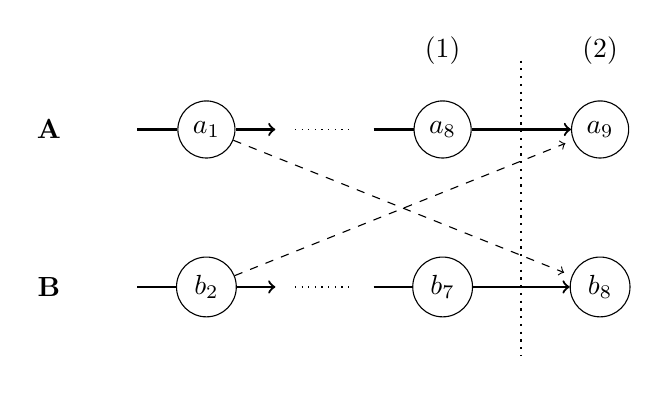
\begin{tikzpicture}
            \path
                node {\textbf{A}}
                to ++(0:1) node (a0) {}
                to ++(0:1) node[op] (a1) {$a_1$}
                to ++(0:1) node (a2) {}
                to ++(0:1) node (a7) {}
                to ++(0:1) node[op] (a8) {$a_8$}
                to ++(90:1) node {(1)}
                to ++(0:1) node (hideTop) {}
                to ++(270:1)
                to ++(0:1) node[op] (a9) {$a_9$}
                to ++(90:1) node {(2)};

            \draw[->, thick] (a0) --  (a1) -- (a2);
            \draw[dotted] (a2) -- (a7);
            \draw[->, thick] (a7) -- (a8) -- (a9);

            \path
                to ++(270:2) node {\textbf{B}}
                to ++(0:1) node (b0) {}
                to ++(0:1) node[op] (b2) {$b_2$}
                to ++(0:1) node (b3) {}
                to ++(0:1) node (b6) {}
                to ++(0:1) node[op] (b7) {$b_7$}
                to ++(0:1)
                to ++(270:1) node (hideBot) {}
                to ++(90:1)
                to ++(0:1) node[op] (b8) {$b_8$};

            \draw[->, thick] (b0) -- (b2) -- (b3);
            \draw[dotted] (b3) -- (b6);
            \draw[->, thick] (b6) -- (b7) -- (b8);

            \draw[->, dashed, shorten >= 3] (a1) -- (b8);
            \draw[->, dashed, shorten >= 3] (b2) -- (a9);

            \draw[dotted, thick] (hideTop) -- (hideBot);
        \end{tikzpicture}
        \label{fig:GC-execution}}
    \hfil
    \subfloat[States of respective epoch trees at (1)]{
        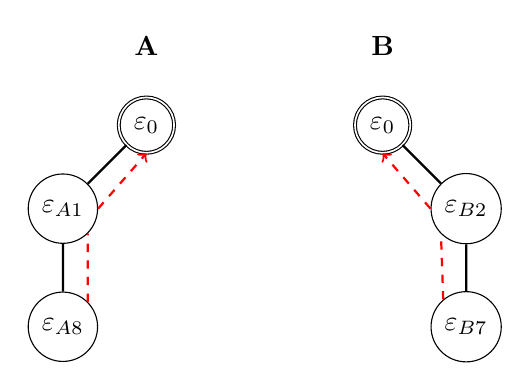
\begin{tikzpicture}
            \path
                node {\textbf{A}}
                to ++(270:1) node[causalop] (AeA0) {\epoch{0}}
                to ++(225:1.5) node[op] (AeA1) {\epoch{A1}}
                to ++(270:1.5) node[op] (AeA8) {\epoch{A8}};

            \path
                to ++(0:3) node {\textbf{B}}
                to ++(270:1) node[causalop] (BeB0) {\epoch{0}}
                to ++(315:1.5) node[op] (BeB2) {\epoch{B2}}
                to ++(270:1.5) node[op] (BeB7) {\epoch{B7}};


            \draw[thick] (AeA0) -- (AeA1) -- (AeA8);
            \draw[thick] (BeB0) -- (BeB2) -- (BeB7);
            \draw[->, dashed, thick, red] (AeA8.45) -- (AeA1.315) (AeA1.0) -- (AeA0.270);
            \draw[->, dashed, thick, red] (BeB7.130) -- (BeB2.225) (BeB2.180) -- (BeB0.270);

        \end{tikzpicture}
        \label{fig:GC-epoch-trees-step-1}}
    \hfil
    \subfloat[States of respective epoch trees at (2)s]{
        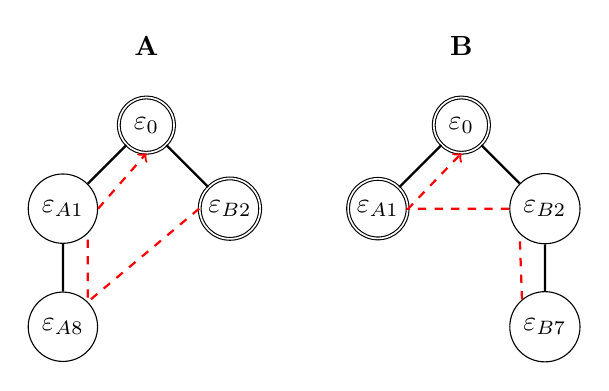
\begin{tikzpicture}
            \path
                node {\textbf{A}}
                to ++(270:1) node[causalop] (Ae0) {\epoch{0}}
                to ++(225:1.5) node[op] (AeA1) {\epoch{A1}}
                to ++(270:1.5) node[op] (AeA8) {\epoch{A8}};
            \path
                to ++(270:1)
                to ++(315:1.5) node[causalop] (AeB2) {\epoch{B2}};

            \path
                to ++(0:4) node {\textbf{B}}
                to ++(270:1) node[causalop] (Be0) {\epoch{0}}
                to ++(315:1.5) node[op] (BeB2) {\epoch{B2}}
                to ++(270:1.5) node[op] (BeB7) {\epoch{B7}};
            \path
                to ++(0:4)
                to ++(270:1)
                to ++(225:1.5) node[causalop] (BeA1) {\epoch{A1}};


            \draw[thick] (Ae0) -- (AeA1) -- (AeA8) (Ae0) -- (AeB2);
            \draw[thick] (Be0) -- (BeB2) -- (BeB7) (Be0) -- (BeA1);
            \draw[->, dashed, thick, red] (AeB2.180) -- (AeA8.45) -- (AeA1.315) (AeA1.0) -- (Ae0.270);
            \draw[->, dashed, thick, red] (BeB7.130) -- (BeB2.225) (BeB2.180) -- (BeA1.0) -- (Be0.270);

        \end{tikzpicture}
        \label{fig:GC-epoch-trees-step-2}}
    \caption{Garbage collecting epochs and corresponding \emph{former states}}
    \label{fig:GC-epochs}
\end{figure}

\mnnote{TODO: Marquer comme GC \epoch{A1} et \epoch{A8} via \autoref{rule:gc-concurrent-primary-epoch} et \epoch{0} via \autoref{rule:gc-root} de l'epoch tree de A dans la \autoref{fig:GC-epoch-trees-step-2}}

\section{Evaluation}

\subsection{Simulations and benchmarks}

In order to validate the proposed approach, we proceed to an experimental evaluation.
The aims of this evaluation are to measure
\begin{enumerate*}[label=(\roman*)]
    \item the memory overhead of the replicated sequence
    \item the computational overhead added to \emph{insert} and \emph{remove} operations by the renaming mechanism
    \item the cost of integrating \emph{rename} operations.
\end{enumerate*}

Unfortunately, we were not able to retrieve an existing dataset of real-time collaborative editing sessions.
We thus setup simulations to generate the dataset used to run our benchmarks.
These simulations mimic the following scenario.

Several authors collaboratively write an article in real-time.
First of all, the authors mainly specify the content of the article.
Few \emph{remove} operations are issued in order to simulate spelling mistakes.
Once the document reaches an arbitrary given critical length, collaborators move on to the second phase of the simulation.
During this phase, authors stop adding new content but instead focus on revamping existing parts.
This is simulated by balancing the ratio between \emph{insert} and \emph{remove} operations.
Every author has to issue a given number of \emph{insert} and \emph{remove} operations.
The simulation ends once every collaborators received all operations.
During the simulation, we take snapshots of the replicas' state at given steps to follow their evolution.

We ran simulations with the following experimental settings: we deployed 10 bots as separate Docker containers on a single workstation.
Each container corresponds to a single mono-threaded Node.js process simulating an author.
Bots share and edit collaboratively the document using either LogootSplit or RenamableLogootSplit according to the session.
In both cases, each bot performs an \emph{insert} or a \emph{remove} operation locally every 200 $\pm$ 50ms and broadcasts it immediately to other nodes using a \ac{P2P} full mesh network.
During the first phase, the probability of issuing \emph{insert} (resp. \emph{remove}) operations is of 80\% (resp. 20\%).
Once the document reaches 60k characters (around 15 pages), bots switch to the second phase and set both probabilities to 50\%.
After each local operation, the bot may move its cursor to another random position in the document with a probability of 5\%.
Every bot generates 15k \emph{insert} or \emph{remove} operations and stops once it observed 150k operations.
Snapshots of the state of bot are taken periodically every 10k observed operations.

Additionally, in the case of RenamableLogootSplit, 1 to 4 bots are arbitrarily designated as \emph{renaming bots} according to the session.
\emph{Renaming bots} issue \emph{rename} operations every time they observe 30k operations overall.
These \emph{rename} operations are generated in a way ensuring that they are concurrent.

Code, benchmarks and results are available at: \url{https://github.com/coast-team/mute-bot-random/}.

\subsection{Results}

\paragraph{Convergence}

We first proceeded to verify the convergence of nodes states at the end of simulations.
For each simulation, we compared the final state of every nodes using their respective snapshots.
We were able to confirm that nodes converged without any communication other than operations, thus satisfying the \ac{SEC} consistency model.

This result sets a first milestone in the validation of the correctness of RenamableLogootSplit.
It is however only empirical.
Further work to formally prove its correctness should be undertaken.

\paragraph{Memory overhead}

\begin{figure}[t!]
    \centering
    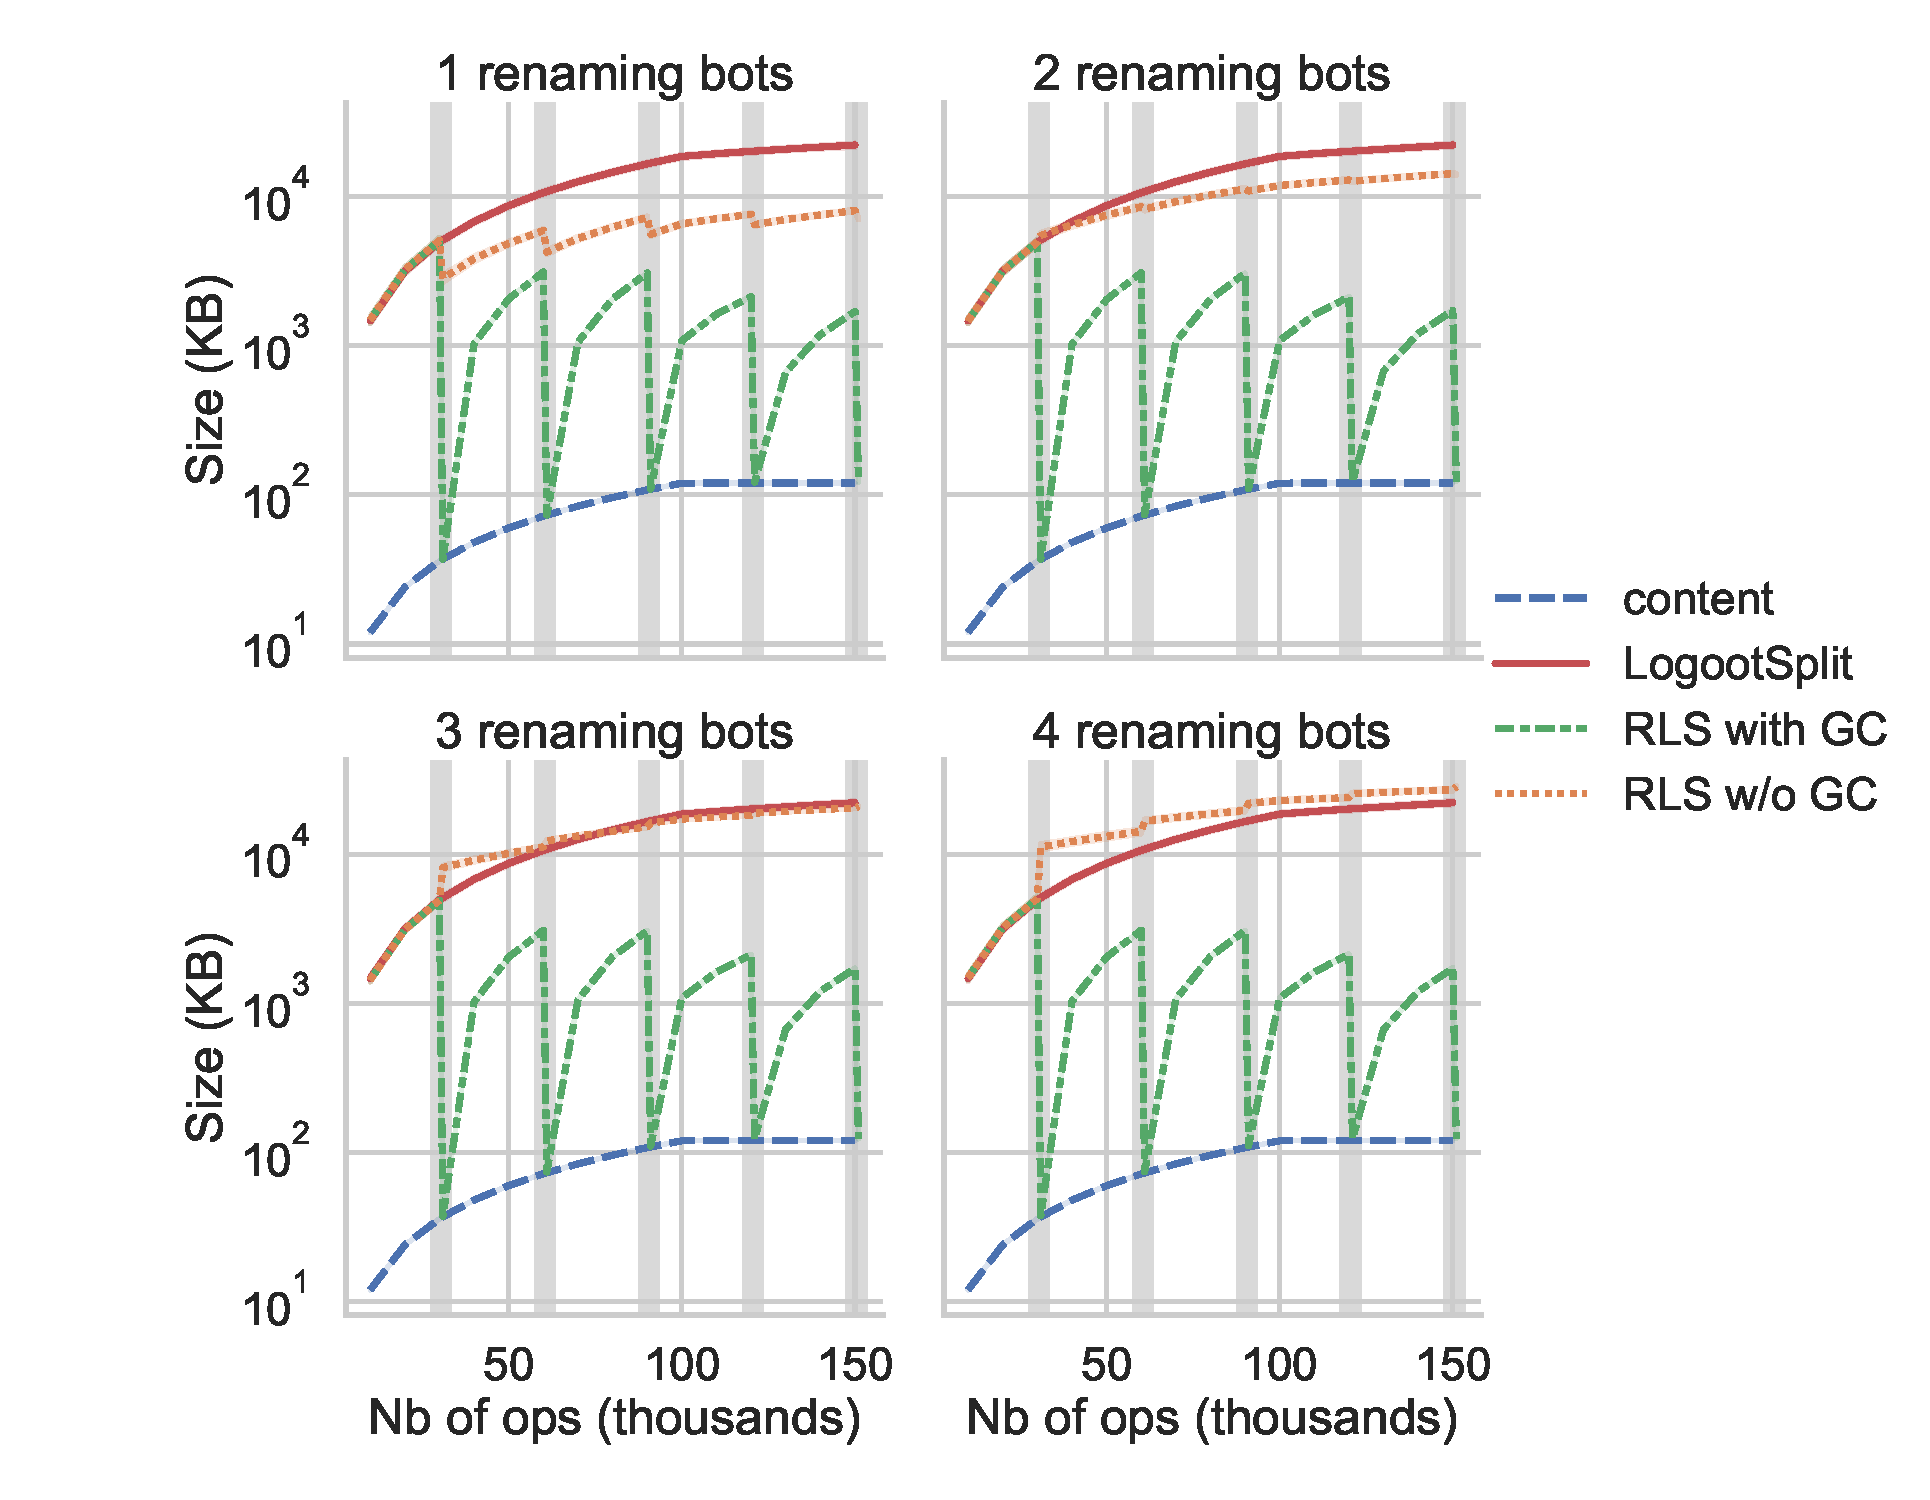
\includegraphics[width=\columnwidth]{img/snapshot-sizes.pdf}
    \caption{Evolution of the size of the document}
    \label{fig:evolution-document-size}
\end{figure}

We then proceeded to measure the evolution of the document's memory consumption throughout the simulations, according to the CRDT used and the number of \emph{renaming bots}.
We present the obtained results in \autoref{fig:evolution-document-size}.

For each plot displayed in \autoref{fig:evolution-document-size}, we represent 4 different data.
The blue dashed line illustrates the size of the actual content of the document, \ie the text, while the red solid line corresponds to the size of the whole LogootSplit document.

The green dashed-dotted line represents the size of the RenamableLogootSplit document in the best case scenario.
In this scenario, nodes assume that \emph{rename} operations are garbage-collectable as soon as they receive them.
Nodes are thus able to benefit the effects of the renaming mechanism while removing its own metadata, such as \emph{former states} and epochs.
In doing so, nodes are able to minimise periodically the metadata overhead of the data structure, independently of the number of \emph{renaming bots} and concurrent \emph{rename} operations issued.

On the other hand, the orange dotted line represents the size of the RenamableLogootSplit document in the worst case scenario.
In this scenario, nodes assume that \emph{rename} operations never become causally stable and can thus never be garbage-collected.
Nodes have to permanently store the metadata introduced by the renaming mechanism.
The performances of RenamableLogootSplit thus decrease as the number of \emph{renaming bots} and \emph{rename} operations issued increases.
Nonetheless, we observe that RenamableLogootSplit can outperform LogootSplit even in this worst case scenario while the number of \emph{renaming bots} remains low (1 or 2).
This result is explained by the fact that the renaming mechanism enables nodes to scrap the overhead of the internal data structure used to represent the document.

To summarise the results presented, the renaming mechanism introduces a temporary metadata overhead which increases with each \emph{rename} operations.
But the overhead will eventually subsides once the system becomes quiescent and \emph{rename} operations become causally stable.
In \autoref{sec:offloading-former-states}, we discuss that \emph{former states} may be offloaded until causal stability is achieved to address the temporary memory overhead.

\paragraph{Integration times of standard operations}

\begin{figure}[t!]
    \centering
    \subfloat[Local operations]{
        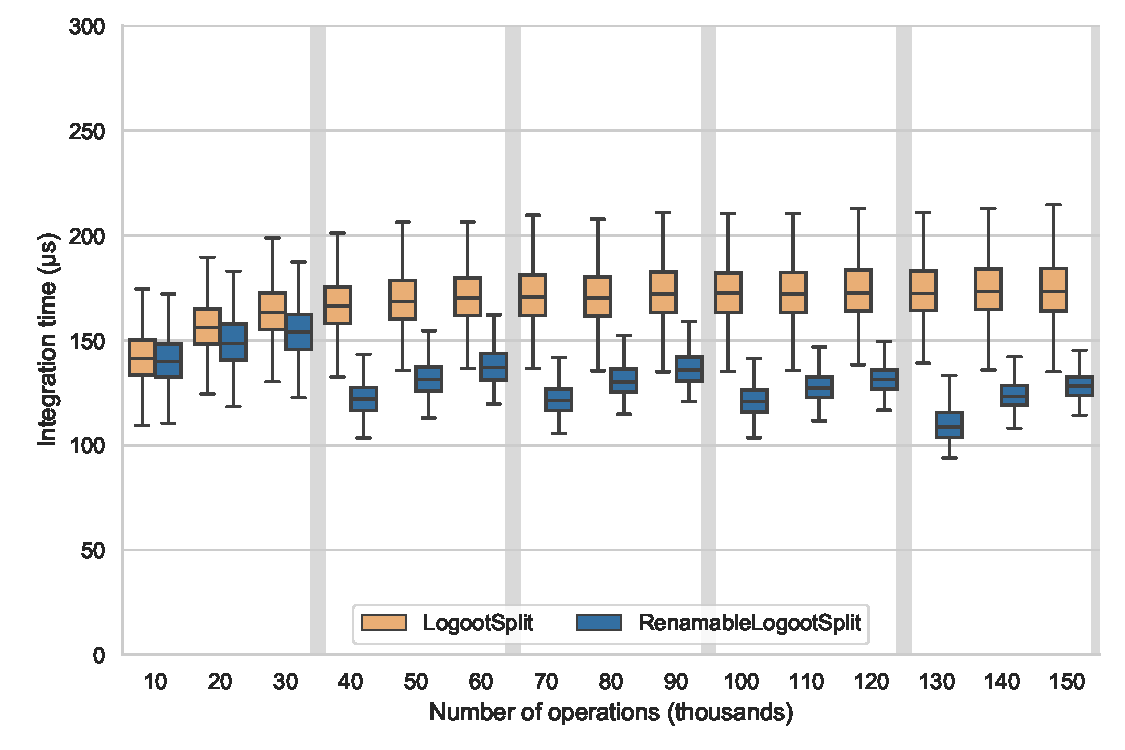
\includegraphics[width=0.9\columnwidth]{img/integration-time-boxplot-local-operations-without-outliers.pdf}
        \label{fig:evolution-integration-time-local-insert}}
    \hfil
    \subfloat[Remote operations]{
        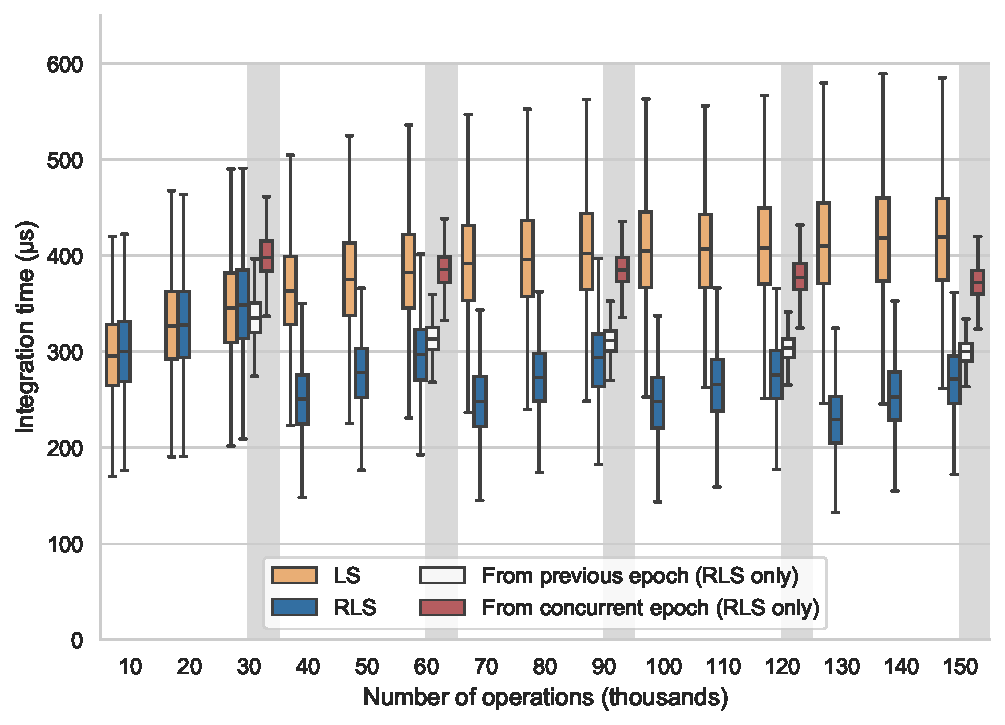
\includegraphics[width=0.9\columnwidth]{img/integration-time-boxplot-remote-operations-without-outliers.pdf}
        \label{fig:evolution-integration-time-remote-insert}}
    \caption{Integration time of standard operations}
    \label{fig:evolution-integration-time-insert}
\end{figure}

Next, we compared the evolution of integration times of respectively local and remote operations on LogootSplit and RenamableLogootSplit documents.
\autoref{fig:evolution-integration-time-insert} displays the results.

In these figures, orange boxplots correspond to integration times on LogootSplit documents while blue ones correspond to times on RenamableLogootSplit documents.
While both are initially equivalent, integration times on RenamableLogootSplit documents are then reduced when compared to LogootSplit ones once \emph{rename} operations have been applied.
This improvement is explained by the fact that \emph{rename} operations optimise the internal representation of the sequence.

Additionally, in the case of remote operations, we measured specific integration times for RenamableLogootSplit : integration times of remote operations from previous epochs and from concurrent epochs, respectively displayed as white and red boxplots in \autoref{fig:evolution-integration-time-remote-insert}.
Operations from previous epochs are operations generated concurrently to the \emph{rename} operation but applied after it.
Since the operation has to be transformed beforehand using \autoref{alg:renameId}, we observe a computational overhead compared to other operations.
But this overhead is actually compensated by the optimisation of the internal representation of the sequence performed by \emph{rename} operations.

Regarding operations from concurrent epochs, we observe an additional overhead as nodes have first to reverse the effect of the concurrent \emph{rename} operation using \autoref{alg:revertRenameId}.
Because of this overhead, RenamableLogootSplit's performances for these operations are comparable to LogootSplit ones.

To summarise, transformation functions introduce an overhead with regard to integration times of concurrent operations to \emph{rename} ones.
Despite this overhead, RenamableLogootSplit achieves better performances than LogootSplit as long as the distance between the epoch of generation of the operation and the current epoch of the node remains limited.
As the distance between both epochs increases, it leads to cases presenting worse performances than LogootSplit ones since the overhead is multiplied.
Nonetheless, the renaming mechanism reduces the integration times of the majority of operations, \ie the operations issued between two rounds of \emph{rename} operations.

\paragraph{Integration time of \emph{rename} operation}

\begin{table}[t!]
    \centering
    \caption{Integration time of rename operations}
    \label{tab:evolution-integration-time-rename}
    \resizebox{\columnwidth}{!}{
        \begin{tabular}{llrrrr}
            \toprule
            \multicolumn{2}{c}{Parameters} & \multicolumn{4}{c}{Integration Time (ms)} \\
            \cmidrule(lr){1-2} \cmidrule(lr){3-6}
            Type & Nb Ops (k) &   Mean &   Median & 99\textsuperscript{th} Quant. &    Std \\
            \midrule
            Local & 30  &    41.75 &    38.74 &      71.68 &   6.84 \\
                                    & 60  &    78.32 &    78.16 &      81.42 &   1.24 \\
                                    & 90  &   119.19 &   118.87 &     124.22 &   2.49 \\
                                    & 120 &   143.75 &   143.57 &     148.59 &   2.16 \\
                                    & 150 &   158.04 &   157.95 &     164.38 &   2.49 \\
            \cmidrule(lr){1-6}
            Remote & 30  &   481.32 &   477.13 &     537.30 &  17.11 \\
                                    & 60  &   981.62 &   978.24 &    1072.83 &  31.54 \\
                                    & 90  &  1491.28 &  1481.83 &    1657.58 &  51.10 \\
                                    & 120 &  1670.00 &  1663.85 &    1814.38 &  50.29 \\
                                    & 150 &  1694.17 &  1675.95 &    1852.55 &  59.94 \\
            \cmidrule(lr){1-6}
            Prim. Remote & 30  &   643.53 &   643.57 &     682.80 &  13.42 \\
                                    & 60  &  1317.66 &  1316.39 &    1399.55 &  28.67 \\
                                    & 90  &  1998.23 &  1994.08 &    2111.98 &  45.37 \\
                                    & 120 &  2239.71 &  2233.22 &    2368.45 &  50.06 \\
                                    & 150 &  2241.92 &  2233.61 &    2351.02 &  52.20 \\
            \cmidrule(lr){1-6}
            Sec. Remote & 30  &     1.36 &     1.30 &       3.53 &   0.37 \\
                                    & 60  &     2.82 &     2.69 &       4.85 &   0.45 \\
                                    & 90  &     4.45 &     4.23 &       5.81 &   0.71 \\
                                    & 120 &     5.33 &     5.10 &       8.78 &   0.90 \\
                                    & 150 &     5.53 &     5.26 &       8.70 &   0.79 \\
            \bottomrule
        \end{tabular}
    }
\end{table}

Finally, we measured the evolution of integration times of \emph{rename} operation according to the number of operations since the last \emph{rename} one.
The results are displayed in \autoref{tab:evolution-integration-time-rename}.

The main outcome of these measures shows that \emph{rename} operations are expensive when compared to others.
Local \emph{rename} operations take hundreds of milliseconds while remote ones and concurrent \emph{primary} ones may last seconds if delayed for too long.
It is thus necessary to take this result into account when designing strategies to trigger \emph{rename} operations to prevent them from impacting negatively user experiences.

Another interesting result from this benchmark is that concurrent \emph{secondary rename} operations are cheap to apply, as they only consist in storage of corresponding \emph{former states}.
Thus nodes can significantly reduce the overall computations of a set of concurrent \emph{rename} operations by applying them in a specific order.
We will discuss further this topic in \autoref{sec:postponing-transition-to-new-epoch}.

\section{Discussion}

\subsection{Offloading on disk unused \emph{former states}}
\label{sec:offloading-former-states}

As explained in \autoref{sec:reverting-rename-op}, nodes have to store \emph{former states} corresponding to \emph{rename} operations to transform operations from previous or concurrent epochs.
Nodes may receive such operations given 2 different cases :
\begin{enumerate*}[label=(\roman*)]
    \item nodes have recently issued \emph{rename} operations
    \item nodes logged back in the collaboration.
\end{enumerate*}
Between these specific events, \emph{former states} are actually not needed to handle operations.

We can thus propose the following trade-off : to offload \emph{former states} on the disk until their next use or until they can be garbage collected.
It would enable nodes to mitigate the temporary memory overhead introduced by the renaming mechanism but increases integration times of operations requiring one of these \emph{former states}.
Nodes could adopt various strategies to deem \emph{former states} offloadable and to retrieve them preemptively according to their constraints.
The design of these strategies could be based on several heuristics : epochs of currently online nodes, number of nodes still able to issue concurrent operations, time elapsed since last use of the \emph{former state}...

\subsection{Designing a more effective \emph{priority} relation}
\label{sec:designing-more-effective-priority-relation}

Although the \emph{priority} relation proposed in \autoref{sec:priority} is simple and ensures that nodes designate the same epoch as the \emph{primary} one, it introduces a significant computational overhead in some cases.
Notably it allows a single node, disjoined from the collaboration since a long time, to force every other nodes to revert \emph{rename} operations they performed meanwhile because its own \emph{rename} operation is deemed as the \emph{primary} one.

The \emph{priority} relation should thus be designed to ensure convergence, but also to minimise the overall amount of computations performed by nodes of the system.
In order to design the \emph{priority} relation, we could embed into \emph{rename} operations metrics that represent the state of the system and the accumulated work on the document (number of nodes currently at the \emph{parent} epoch, number of operations generated at the \emph{parent epoch}, length of the document...).
This way, we can favour the branch from the \emph{epoch tree} with the more and most active collaborators and prevent isolated nodes from overthrowing the existing order.

\subsection{Postponing transition to \emph{primary} epoch in case of high concurrency}
\label{sec:postponing-transition-to-new-epoch}

As shown in \autoref{tab:evolution-integration-time-rename}, integrating \emph{primary rename} operations is expensive as nodes have to browse and rename their whole current state.
This process can introduce a signification computational overhead in some cases.
Especially, a node may receive concurrent \emph{rename} operations in the reverse order to the one defined by the \emph{priority} relation.
In this scenario, the node would successively consider every \emph{rename} operation as the \emph{primary} one and would rename its state each time.
On the other hand \emph{secondary rename} operations are cheap to integrate, as nodes simply add to their state a reference to the corresponding \emph{former state}.

To mitigate the negative impact of this scenario, we can decompose the integration of \emph{rename} operations into two parts in case of concurrency detection.
First, nodes process \emph{rename} operations as secondary ones.
It enables nodes to integrate remote \emph{insert} and \emph{remove} operations, even from concurrent epochs, by transforming them.
Then each node keeps track of a level of confidence in the current \emph{primary} operation, computed for example from the time elapsed since the node received a concurrent \emph{rename} operation and the number of online nodes still known as using the \emph{parent} epoch.
Once the level of confidence reaches a given threshold, the node renames its state according to the operation.

This strategy introduces a slight computational overhead for each \emph{insert} or \emph{remove} operations received during the period of uncertainty, as nodes may issue operations from different epochs during that time.
In return, the strategy reduces the probability of erroneously integrating \emph{rename} operations as \emph{primary} ones.

\section{Related work}

Several works were proposed to address our problem of growth of identifiers in variable-size identifiers Sequence \acp{CRDT}.
We present in this section the most relevant ones.

\subsection{The core-nebula approach}

The \emph{core-nebula} approach \cite{letia:hal-01248270, zawirski:hal-01248197} was proposed to reduce the size of identifiers in Treedoc\cite{5158449}, another variable-size identifiers Sequence \ac{CRDT}.

In this work, authors introduce a \emph{rebalance} operation enabling nodes to reassign shorter identifiers to elements of the document.
However, this \emph{rebalance} operation is not commutative with \emph{insert} and \emph{remove} operations nor with itself.
To achieve \ac{EC}\cite{10.1145/224057.224070}, the \emph{core-nebula} approach prevents concurrent \emph{rebalance} operations by regulating them using a consensus protocol.
Operations such as \emph{insert} and \emph{remove} can still be issued without coordination and can thus be concurrent to \emph{rebalance} ones.
To deal with this issue, authors propose a \emph{catch-up} protocol to transform these concurrent operations against the effects of \emph{rebalance} ones.

Since consensus protocols do not scale well, the \emph{core-nebula} approach proposes to split nodes among two groups : the \emph{core} and the \emph{nebula}.
The \emph{core} is a small set of stable and highly connected nodes while the \emph{nebula} is an unbounded set of dynamic nodes.
Only nodes from the \emph{core} participate in the execution of the consensus protocol.
Nodes from the \emph{nebula} can still contribute to the document by issuing \emph{insert} and \emph{remove} operations.

Our work can be seen as an extension of this work.
It adapts the \emph{rebalance} mechanism and the \emph{catch-up} protocol to LogootSplit and takes advantage of its block feature.
Furthermore, it integrates a mechanism to deal with concurrent \emph{rename} operations, hence removing the requirement of a consensus protocol.
It makes this approach usable in systems without existing authorities providing nodes to the \emph{core}.

However, systems can actually adopt the \emph{core-nebula} approach to simplify the implementation of RenamableLogootSplit.
The use of a consensus protocol to regulate \emph{rename} operations enables systems to discard all parts dedicated to the handling of concurrent \emph{rename} operations, \ie the design of a \emph{priority} relation and the implementation of \autoref{alg:revertRenameId} and \autoref{rule:gc-concurrent-primary-epoch}.

\subsection{The LSEQ approach}

The LSEQ approach \cite{nedelec_2013_lseq, doi:10.1002/cpe.4108} is another approach proposed to address the growth of identifiers in variable-size identifiers Sequence \ac{CRDT}. Instead of reducing periodically the identifier metadata using an expensive renaming mechanism, the authors define new identifier allocation strategies to reduce their growth rate.

In this work, authors observe that the identifier allocation strategy proposed in Logoot\cite{WeissICDCS09} is suited to a single editing pattern : from left to right, top to bottom.
If insertions are made according to other patterns, generated identifiers quickly saturate the space of possible identifiers for a given size.
Following insertions therefore trigger an increase of the identifier size.
As a result, Logoot identifiers grow linearly with the number of insertions instead of the expected logarithmic progression.

LSEQ thus defines several identifier allocation strategy fitted to different editing pattern.
Nodes pick randomly one of these strategies for each identifier size.
Additionally LSEQ adopts an exponential tree model for identifiers : the range of possible identifiers doubles as the identifier size increases.
\mnnote{TODO: Voir comment mieux formuler ce passage sur le nombre de bits alloués à \emph{position} qui double à chaque "profondeur" d'identifiant.}
It enables LSEQ to fine-tune the size of identifiers according to needs.
By combining the different allocation strategies to the exponential tree model, LSEQ achieves a polylogarithmic growth of identifiers according to the number of insertions.

While the LSEQ approach reduces the growth rate of identifiers in variable-size identifier Sequence \ac{CRDT}, the sequence's overhead is still proportional to its number of elements.
On the other hand, RenamableLogootSplit's renaming mechanism enables to reduce metadata to a fixed amount, independently of the number of elements.

These two approaches are actually orthogonal and can, as in the previous approach, be combined.
The resulting system would reset the sequence's metadata periodically using \emph{rename} operations while LSEQ's identifier allocation strategies would reduce their growth in-between.
This would also enable to reduce the frequency of \emph{rename} operations, decreasing the system computations overall.

\section{Conclusions and future work}

The conclusion goes here.


% if have a single appendix:
%\appendix[Proof of the Zonklar Equations]
% or
%\appendix  % for no appendix heading
% do not use \section anymore after \appendix, only \section*
% is possibly needed

% use appendices with more than one appendix
% then use \section to start each appendix
% you must declare a \section before using any
% \subsection or using \label (\appendices by itself
% starts a section numbered zero.)
%


\appendices
\section{Proof of the First Zonklar Equation}
Appendix one text goes here.

% you can choose not to have a title for an appendix
% if you want by leaving the argument blank
\section{}
Appendix two text goes here.

\section*{Acknowledgments}

The authors would like to thank...


% Can use something like this to put references on a page
% by themselves when using endfloat and the captionsoff option.
\ifCLASSOPTIONcaptionsoff
  \newpage
\fi



% trigger a \newpage just before the given reference
% number - used to balance the columns on the last page
% adjust value as needed - may need to be readjusted if
% the document is modified later
%\IEEEtriggeratref{8}
% The "triggered" command can be changed if desired:
%\IEEEtriggercmd{\enlargethispage{-5in}}

% references section

\bibliographystyle{IEEEtran}
\bibliography{ref}

% biography section
%
% If you have an EPS/PDF photo (graphicx package needed) extra braces are
% needed around the contents of the optional argument to biography to prevent
% the LaTeX parser from getting confused when it sees the complicated
% \includegraphics command within an optional argument. (You could create
% your own custom macro containing the \includegraphics command to make things
% simpler here.)
%\begin{IEEEbiography}[{\includegraphics[width=1in,height=1.25in,clip,keepaspectratio]{mshell}}]{Michael Shell}
% or if you just want to reserve a space for a photo:

\begin{IEEEbiography}{Michael Shell}
Biography text here.
\end{IEEEbiography}

% if you will not have a photo at all:
\begin{IEEEbiographynophoto}{John Doe}
Biography text here.
\end{IEEEbiographynophoto}

% insert where needed to balance the two columns on the last page with
% biographies
%\newpage

\begin{IEEEbiographynophoto}{Jane Doe}
Biography text here.
\end{IEEEbiographynophoto}

% You can push biographies down or up by placing
% a \vfill before or after them. The appropriate
% use of \vfill depends on what kind of text is
% on the last page and whether or not the columns
% are being equalized.

%\vfill

% Can be used to pull up biographies so that the bottom of the last one
% is flush with the other column.
%\enlargethispage{-5in}

\end{document}
